% Created 2024-01-28 Sun 19:52
% Intended LaTeX compiler: pdflatex
\documentclass[presentation]{beamer}
\usepackage[utf8]{inputenc}
\usepackage[T1]{fontenc}
\usepackage{graphicx}
\usepackage{longtable}
\usepackage{wrapfig}
\usepackage{rotating}
\usepackage[normalem]{ulem}
\usepackage{amsmath}
\usepackage{amssymb}
\usepackage{capt-of}
\usepackage{hyperref}
\mode<beamer>{\usetheme{Madrid}}
\definecolor{SUred}{rgb}{0.59375, 0, 0.17969} % SU red (primary)
\definecolor{SUblue}{rgb}{0, 0.17578, 0.38281} % SU blue (secondary)
\setbeamercolor{palette primary}{bg=SUred,fg=white}
\setbeamercolor{palette secondary}{bg=SUblue,fg=white}
\setbeamercolor{palette tertiary}{bg=SUblue,fg=white}
\setbeamercolor{palette quaternary}{bg=SUblue,fg=white}
\setbeamercolor{structure}{fg=SUblue} % itemize, enumerate, etc
\setbeamercolor{section in toc}{fg=SUblue} % TOC sections
% Override palette coloring with secondary
\setbeamercolor{subsection in head/foot}{bg=SUblue,fg=white}
\setbeamercolor{date in head/foot}{bg=SUblue,fg=white}
\institute[SU]{Shenandoah University}
\titlegraphic{\includegraphics[width=0.5\textwidth]{\string~/Documents/suLogo/suLogo.pdf}}
\newcommand{\R}{\mathbb{R}}
\usepackage{tikz}
\usetheme{default}
\author{Chase Mathison\thanks{cmathiso@su.edu}}
\date{29 January 2024}
\title{The Unit Circle: Sines and Cosines}
\hypersetup{
 pdfauthor={Chase Mathison},
 pdftitle={The Unit Circle: Sines and Cosines},
 pdfkeywords={},
 pdfsubject={},
 pdfcreator={Emacs 29.1 (Org mode 9.6.7)}, 
 pdflang={English}}
\begin{document}

\maketitle

\section{Announcements}
\label{sec:org13e4d91}
\begin{frame}[label={sec:org469123f}]{Announcements}
\begin{enumerate}
\item Homework in MyOpenMath!
\item Office hours, 10am - 11am.
\end{enumerate}
\end{frame}

\section{Lecture}
\label{sec:orgb9f5180}
\begin{frame}[label={sec:orgf72f3a6}]{The Unit Circle}
\begin{block}{Definitions}
\begin{itemize}
\item Unit Circle
\end{itemize}
\end{block}


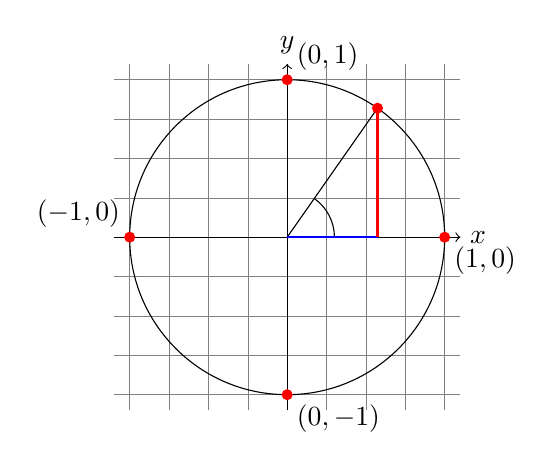
\begin{tikzpicture}[scale=2]
  \draw[help lines,step=0.25] (-1.1,-1.1) grid (1.1,1.1);
  \draw[->] (-1.1,0) -- (1.1,0) node[anchor=west] {$x$};
  \draw[->] (0,-1.1) -- (0,1.1) node[anchor=south] {$y$};
  \draw (0,0) circle [radius=1];
  \node at (1,0) [anchor=north west] {$(1,0)$};
  \fill[color=red] (1,0) circle [radius=1pt];
  \node at (0,1) [anchor=south west] {$(0,1)$};
  \fill[color=red] (0,1) circle [radius=1pt];
  \node at (0,-1) [anchor=north west] {$(0,-1)$};
  \fill[color=red] (0,-1) circle [radius=1pt];
  \node at (-1,0) [anchor=south east] {$(-1,0)$};
  \fill[color=red] (-1,0) circle [radius=1pt];
  \draw[color=black] (0,0) -- (55:1);
  \draw (0,0) -- (0.3,0)  arc [start angle = 0, end angle=55, radius=0.3];
  \fill[color=red] (55:1) circle [radius=1pt];
  \draw[color=blue,thick] (0,0) -- (55:1 |- 0,0);
  \draw[color=red,thick] (0,0) ++(55:1) -- (55:1 |- 0,0);
\end{tikzpicture}
\end{frame}

\begin{frame}[label={sec:org8be5ad9}]{The Unit Circle}
\begin{block}{Definitions}
If \(\theta\) is an angle measure and \(\left( x,y \right)\) is the
point on the unit circle corresponding to an angle of \(\theta\), then
\vspace{0.2in}
\end{block}

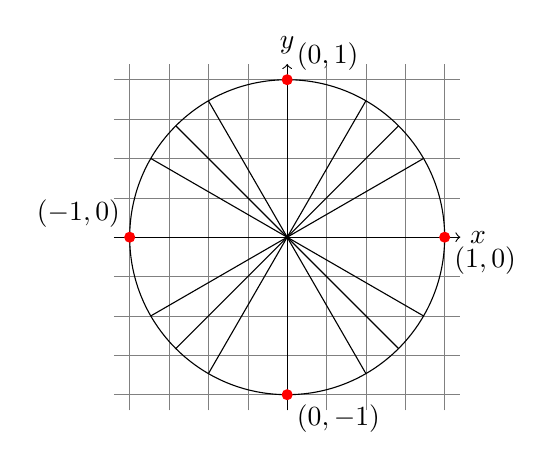
\begin{tikzpicture}[scale=2]
  \draw[help lines,step=0.25] (-1.1,-1.1) grid (1.1,1.1);
  \draw[->] (-1.1,0) -- (1.1,0) node[anchor=west] {$x$};
  \draw[->] (0,-1.1) -- (0,1.1) node[anchor=south] {$y$};
  \draw (0,0) circle [radius=1];
  \node at (1,0) [anchor=north west] {$(1,0)$};
  \fill[color=red] (1,0) circle [radius=1pt];
  \node at (0,1) [anchor=south west] {$(0,1)$};
  \fill[color=red] (0,1) circle [radius=1pt];
  \node at (0,-1) [anchor=north west] {$(0,-1)$};
  \fill[color=red] (0,-1) circle [radius=1pt];
  \node at (-1,0) [anchor=south east] {$(-1,0)$};
  \fill[color=red] (-1,0) circle [radius=1pt];
  \draw (30:-1) -- (30:1);
  \draw (45:-1) -- (45:1);
  \draw (60:-1) -- (60:1);
  \draw (-30:-1) -- (-30:1);
  \draw (-45:-1) -- (-45:1);
  \draw (-60:-1) -- (-60:1);
\end{tikzpicture}
\end{frame}

\begin{frame}[label={sec:org347b33b}]{The Pythagorean Identity}
\begin{block}{Definitions}
\begin{itemize}
\item Pythagorean identity
\end{itemize}
\end{block}


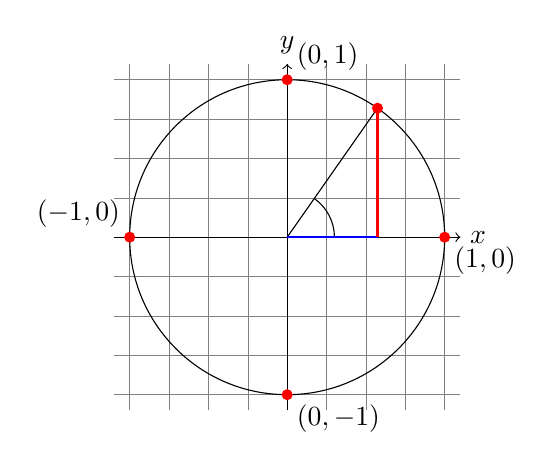
\begin{tikzpicture}[scale=2]
  \draw[help lines,step=0.25] (-1.1,-1.1) grid (1.1,1.1);
  \draw[->] (-1.1,0) -- (1.1,0) node[anchor=west] {$x$};
  \draw[->] (0,-1.1) -- (0,1.1) node[anchor=south] {$y$};
  \draw (0,0) circle [radius=1];
  \node at (1,0) [anchor=north west] {$(1,0)$};
  \fill[color=red] (1,0) circle [radius=1pt];
  \node at (0,1) [anchor=south west] {$(0,1)$};
  \fill[color=red] (0,1) circle [radius=1pt];
  \node at (0,-1) [anchor=north west] {$(0,-1)$};
  \fill[color=red] (0,-1) circle [radius=1pt];
  \node at (-1,0) [anchor=south east] {$(-1,0)$};
  \fill[color=red] (-1,0) circle [radius=1pt];
  \draw[color=black] (0,0) -- (55:1);
  \draw (0,0) -- (0.3,0)  arc [start angle = 0, end angle=55, radius=0.3];
  \fill[color=red] (55:1) circle [radius=1pt];
  \draw[color=blue,thick] (0,0) -- (55:1 |- 0,0);
  \draw[color=red,thick] (0,0) ++(55:1) -- (55:1 |- 0,0);
\end{tikzpicture}
\end{frame}

\begin{frame}[label={sec:orgf1591d8}]{Example}
Suppose \(0 \le \theta \le \pi/2\) and \(\sin(\theta) = \frac{3}{5}\).  What is
\(\cos(\theta)\)?

\vspace{10in}
\end{frame}

\begin{frame}[label={sec:orgbaa423e}]{Example}
Suppose \(\pi \le \theta \le \frac{3\pi}{2}\) and \(\cos(\theta) = -\frac{1}{8}.\) What is
\(\sin(\theta)\)?

\vspace{10in}
\end{frame}
\end{document}